%% ma: L12-B16-0015
%% lop: 12
%% chuong: 5
%% bai: 16
%% dang: 12.16.12
%% loai: TN4
%% muc: VDC
%% dap_an: "D"
%% nguon: "Ảnh giáo viên gửi 04/11/2026 (Huỳnh Văn Ánh, Chuyên đề V - Phương pháp tọa độ trong không gian), Đề test theo bài, Phần I Câu 6"
%% kien_thuc: "Bài 16 (góc giữa đường thẳng và mặt phẳng), Bài 14 (vectơ pháp tuyến), Bài 15 (đường thẳng song song mặt phẳng), Bài 1 và Bài 2 (đạo hàm, bảng biến thiên, giá trị lớn nhất của hàm số)"
%% trang_thai: chinh-thuc
%% ghi_chu: "Đáp án gốc D khớp (sympy): f(m) lớn nhất bằng 5 tại m=0, f(-5/4)=0, giới hạn 16/5. Bảng biến thiên của gốc nằm trong lời giải nên được dựng lại bằng tkz-tab trong lời giải. Đã duyệt 04/11/2026."
\begin{ex}
Trong không gian $Oxyz$, cho mặt phẳng $(P)\colon 2x-y+2z-1=0$ và mặt phẳng $(Q)\colon 4x-4y+3z-2=0$. Đường thẳng $\Delta$ song song với mặt phẳng $(P)$, có một vectơ chỉ phương $\vec u=(m;n;1)$. Khi $\Delta$ tạo với $(Q)$ một góc lớn nhất thì $\sin$ của góc tạo bởi đường thẳng $\Delta$ và mặt phẳng $(Q)$ bằng bao nhiêu?
\choice{$\dfrac{2\sqrt{41}}{41}$}{$1$}{$\dfrac{\sqrt{41}}{41}$}{\True $\dfrac{\sqrt{205}}{41}$}
\loigiai{$(P)$ có vectơ pháp tuyến $\vec n_P=(2;-1;2)$, $(Q)$ có vectơ pháp tuyến $\vec n_Q=(4;-4;3)$.

Vì $\Delta\parallel(P)$ nên $\vec u\perp\vec n_P\Rightarrow2m-n+2=0\Leftrightarrow n=2m+2$.

Khi đó
\[\sin(\Delta,(Q))=\dfrac{|\vec u\cdot\vec n_Q|}{|\vec u|\cdot|\vec n_Q|}=\dfrac{|4m-4n+3|}{\sqrt{m^2+n^2+1}\cdot\sqrt{41}}=\dfrac{|4m+5|}{\sqrt{41}\cdot\sqrt{5m^2+8m+5}}.\]
Suy ra $\sin(\Delta,(Q))=\dfrac1{\sqrt{41}}\sqrt{\dfrac{16m^2+40m+25}{5m^2+8m+5}}$.

Vì $0^\circ\le(\Delta,(Q))\le90^\circ$ nên góc lớn nhất khi $\sin(\Delta,(Q))$ lớn nhất, tức $f(m)=\dfrac{16m^2+40m+25}{5m^2+8m+5}$ lớn nhất.

Ta có $f'(m)=\dfrac{-72m^2-90m}{(5m^2+8m+5)^2}$, $f'(m)=0\Leftrightarrow m=-\dfrac54$ hoặc $m=0$.
\begin{center}
\begin{tikzpicture}
\tkzTabInit[lgt=1.4,espcl=2.8]{$m$/1.2,$f'(m)$/0.8,$f(m)$/1.8}{$-\infty$,$-\dfrac54$,$0$,$+\infty$}
\tkzTabLine{,-,z,+,z,-,}
\tkzTabVar{+/$\dfrac{16}5$,-/$0$,+/$5$,-/$\dfrac{16}5$}
\end{tikzpicture}
\end{center}
Từ bảng biến thiên, $\max f(m)=5$ tại $m=0$. Vậy $\sin(\Delta,(Q))$ lớn nhất bằng
\[\dfrac1{\sqrt{41}}\cdot\sqrt5=\dfrac{\sqrt{205}}{41}.\]
Chọn D.}
\end{ex}
